\documentclass[a4paper, 12pt]{article}

\usepackage{ctex}
\usepackage{graphicx}
\usepackage{amsmath}
\usepackage{geometry}
\usepackage{mathptmx}
\usepackage[T1]{fontenc}
\usepackage{fancyvrb}
\geometry{left=2.0cm, right=2.0cm, top=1.5cm, bottom=1.5cm}   %页边距

\usepackage{tikz}
\usetikzlibrary{graphs, positioning, quotes, shapes.geometric, calc}
% 流程图定义基本形状
\tikzstyle{startstop} = [rectangle, rounded corners, minimum width = 1.6cm, minimum height=0.8cm,text centered, draw = black]
\tikzstyle{io} = [trapezium, trapezium left angle=70, trapezium right angle=110, minimum width=1.6cm, minimum height=0.8cm, text centered, draw=black]
\tikzstyle{process} = [rectangle, minimum width=2.4cm, minimum height=0.8cm, text centered, draw=black]
\tikzstyle{decision} = [diamond, aspect = 3, text centered, draw=black]
% 箭头形式
\tikzstyle{arrow} = [->, ,>=stealth]
\tikzstyle{every node}=[scale=0.7]

\renewcommand{\figurename}{Fig}

\title{\textbf{Report of lab2}}
\author{孟澍 \\ 3210101819}

\begin{document}
\maketitle

\section{Algorithm explanation}
This is the flowchart of my program.

Basic idea: Store the number to be converted in R3, convert each 4-bit into hexadecimal then output.
\begin{figure}[htbp]
  \centering

  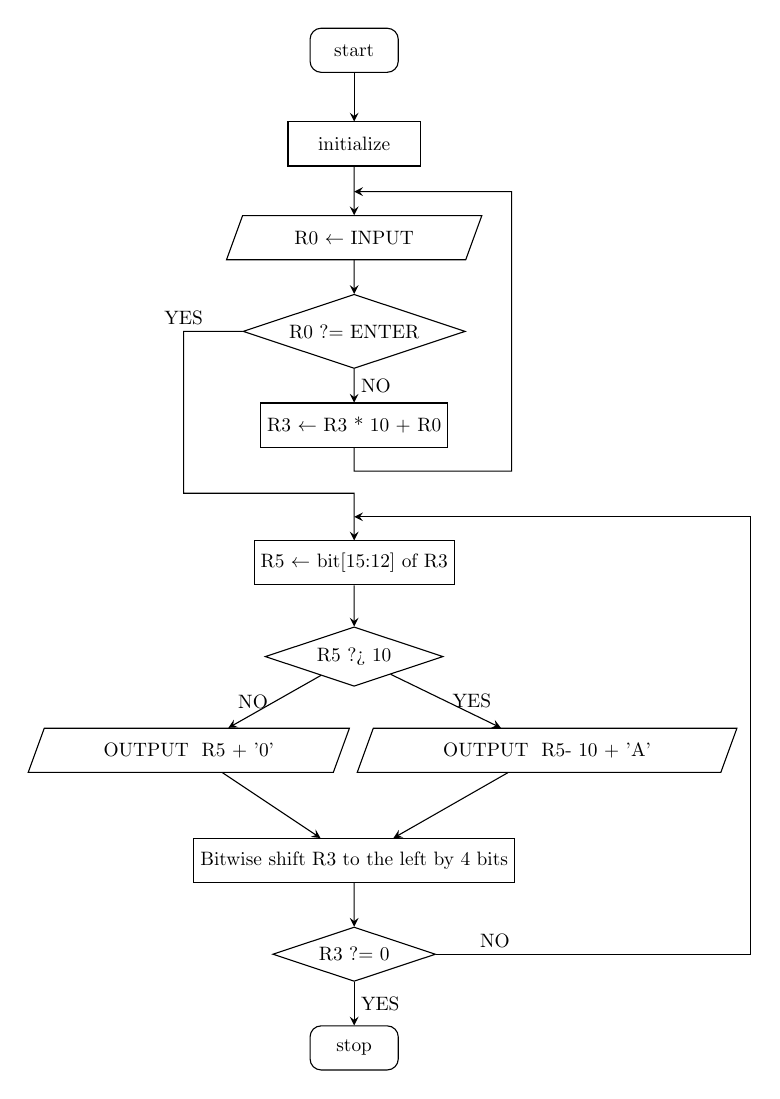
\begin{tikzpicture}[node distance=1.5cm, align=center]
  %定义流程图具体形状
  \node (start) [startstop] {start};
  \node (pro1) [process, below of=start, yshift= -0.2cm] {initialize};
  \node (in1) [io, below of = pro1, yshift = -0.2cm] {R0 $\leftarrow$ INPUT};
  \node (dec1) [decision, below of=in1, yshift= -0.2cm] {R0 ?= ENTER};
  \node (pro2) [process, below of=dec1, yshift= -0.2cm] {R3 $\leftarrow$ R3 * 10 + R0};
  \node (pro3) [process, below of=pro2, yshift = -1cm] {R5 $\leftarrow$ bit[15:12] of R3};
  \node (dec2) [decision, below of=pro3, yshift= -0.2cm] {R5 ?> 10};
  \node (out1) [io, below of=dec2, yshift = -0.2cm, xshift = -3cm] {OUTPUT \ R5 + '0'};
  \node (out2) [io, below of=dec2, yshift = -0.2cm, xshift = 3.5cm] {OUTPUT \ R5- 10 + 'A'};
  \node (pro4) [process, below of=out1, yshift = -0.5cm, xshift = 3cm] {Bitwise shift R3 to the left by 4 bits};
  \node (dec3) [decision, below of=pro4, yshift= -0.2cm] {R3 ?= 0};
  \node (stop) [startstop, below of=dec3, yshift= -0.2cm] {stop};

  %连接具体形状
  \draw [arrow](start) -- (pro1);
  \draw [arrow](pro1) -- (in1);
  \draw [arrow](in1) -- (dec1);
  \draw [arrow](dec1) -- ($(dec1.west) + (-0.75,0)$) node[anchor=south] {YES} |- ($(pro3.north) + (0, 0.6)$) -- (pro3);
  \draw [arrow](dec1) -- node[anchor=west] {NO} (pro2);
  \draw [arrow](pro2) -- ($(pro2.south) + (0, -0.3)$) -- ($(pro2.south) + (2, -0.3)$) -- ($(in1.north) + (2, 0.3)$) -- ($(in1.north) + (0, 0.3)$);
  \draw [arrow](pro3) -- (dec2);
  \draw [arrow](dec2) -- node[anchor=east] {NO} (out1);
  \draw [arrow](dec2) -- node[anchor=west] {YES} (out2);
  \draw [arrow](out1) -- (pro4);
  \draw [arrow](out2) -- (pro4);
  \draw [arrow](pro4) -- (dec3);
  \draw [arrow](dec3) -- ($(dec3.east) + (0.75,0)$) node[anchor=south] {NO} -- ($(dec3.east) + (4,0)$) |- ($(pro3.north) + (0, 0.3)$);
  \draw [arrow](dec3) -- node[anchor = west] {YES} (stop);
  \end{tikzpicture}
\caption{The flowchart of the program.}
\end{figure}

\section{Source code}
\linespread{0.8}      %行距缩小
\begin{Verbatim}[frame = single, numbers = left]
.orig x3000
; initialize
AND R0, R0, #0
AND R4, R4, #0
AND R5, R5, #0
AND R6, R6, #0

LD R1, ZERO
NOT R1, R1
ADD R1, R1, #1   ; R1 <- -'0'

LD R2, RETURN
NOT R2, R2
ADD R2, R2, #1   ; R2 <- -'\r'

AND R3, R3, #0   ; R3 store the number to be converted

INPUT GETC       ; R0 <- inputchar
OUT
ADD R6, R0, R2   ; test R0 ?= '\r'
BRz CONVERT
ADD R0, R0, R1
JSR MUL
BR INPUT

MUL AND R6, R6, #0
ADD R6, R6, #10
AND R5, R5, #0
ADD R5, R5, R3
AND R3, R3, #0
ADD R3, R3, R5       ; R3 <- R3 * 10
ADD R6, R6, #-1
BRp #-3
ADD R3, R3, R0       ; R3 <- R3 + R0
RET

CONVERT ADD R6, R6, #4
BR OUTPUT
CONT ADD R3, R3, R3
ADD R3, R3, R3
ADD R3, R3, R3
ADD R3, R3, R3
ADD R6, R6, #-1
BRp #-7
HALT

; get hexadecimal digit of the current highest 4-bit of R3
; the result is stored in R5
GETHEX LD R1, A
AND R2, R2, #0
ADD R2, R2, #1
AND R5, R5, #0
AND R4, R4, #0
AND R4, R1, R3
BRz #5
NOT R2, R2
NOT R5, R5
AND R5, R5, R2
NOT R5, R5
NOT R2, R2
ADD R2, R2, R2
ADD R1, R1, R1
BRz #1
BR #-12
RET

OUTPUT JSR GETHEX
ADD R5, R5, #-10
BRzp #4
LD R0, ZERO
ADD R0, R0, R5
ADD R0, R0, #10
BR #2
LD R0, CAPA
ADD R0, R0, R5
OUT
BR CONT

RETURN .fill x000A     ; ASCII code of ENTER
ZERO .fill x0030       ; ASCII code of '0'
CAPA .fill x0041  ; ASCII code of 'A'
LOWX .fill x0078    ; ASCII code of 'x'
A .fill x1000
.end
\end{Verbatim}
\linespread{0.9}      %行距恢复

\section{Questions TA asked you and your answer in check}
Question: What's the actual process of the JSR instruction?

First, the address of the instruction following JSR is stored in a temorary location.

Question: 在函数调用时如何保存之前寄存器的值


\end{document}